\documentclass[prl,twocolumn]{revtex4-1}

\usepackage{graphicx}
\usepackage{color}
\usepackage{latexsym,amsmath}
\usepackage[subtle]{savetrees} %questa è la svolta
\definecolor{linkcolor}{rgb}{0,0,0.65} %hyperlink
\usepackage[pdftex,colorlinks=true, pdfstartview=FitV, linkcolor= linkcolor, 
    citecolor= linkcolor, urlcolor= linkcolor, hyperindex=true,hyperfigures=true]{hyperref} %hyperlink%

% Ensure Arabic section numbering instead of Roman numerals
\renewcommand{\thesection}{\arabic{section}}
\renewcommand{\thesubsection}{\thesection.\arabic{subsection}}

\makeatletter
\renewcommand{\section}{\@startsection{section}{1}{\z@}%
    {-3.5ex \@plus -1ex \@minus -.2ex}{2.3ex \@plus.2ex}%
    {\normalfont\bfseries\raggedright}}

\renewcommand{\subsection}{\@startsection{subsection}{2}{\z@}%
    {3.5ex \@plus 1ex \@minus .2ex}{-1em}%
    {\normalfont\bfseries\raggedright}}
\makeatother

\begin{document}

\setcounter{secnumdepth}{1}

\title{Unsupervised Learning and Log-likelihood Analysis with Restricted Boltzmann Machines}

\author{Elias Maria Bonasera}
\author{Alberto Casellato}
\author{Nicola Garbin}
\author{Francesco Pazzocco}

\date{\today}

\begin{abstract}
\textit{We present a comprehensive study on the use of restricted Boltzmann machines (RBMs) for unsupervised learning of handwritten digit features from the MNIST dataset. Through experiments with a custom Python implementation, we focus on the RBM architecture, the training via Contrastive Divergence, and extensive hyperparameter tuning. We detail the experimental setup, the log-likelihood estimation method, and evaluate different configurations. The results highlight both the strengths and limitations of the approach, suggesting directions for future improvements.}
\end{abstract}

\maketitle

%%%%%%%%%%%%%%%%%%%%%%%%%%%%%%%%%%%%%%%%%%%%%%%%%%%%%%%%%%%%%%%%%%%%%%
% 1. Introduction
%%%%%%%%%%%%%%%%%%%%%%%%%%%%%%%%%%%%%%%%%%%%%%%%%%%%%%%%%%%%%%%%%%%%%%
\section*{Introduction}
Unsupervised learning is essential for extracting features from unlabeled data, and probabilistic graphical models (PGMs), such as Markov Random Fields (MRFs), provide a framework for this task. Restricted Boltzmann Machines (RBMs) are a specific type of MRF with a bipartite structure (a visible and a hidden layer with no intra-layer connections). Their ability to model complex distributions and learn efficient representations of intricate data relatively fast makes them interesting both theoretically and for practical applications \cite{intro_ML,bortoletto, practical}.

In this work, we present a complete implementation of a Restricted Boltzmann Machine (RBM) and analyze its behavior through systematic experiments. The paper is organized as follows:
Section~\ref{sec:theory} presents the theoretical foundation of RBMs, Section~\ref{sec:methodology} details the experimental methodology and implementation specifics, Section~\ref{sec:results} shows the experimental results accompanied by graphical analysis, and Section~\ref{sec:discussion} discusses our findings, draws conclusions, and suggests avenues for future research. Supplementary equations and technical details are provided in the Appendix.

%%%%%%%%%%%%%%%%%%%%%%%%%%%%%%%%%%%%%%%%%%%%%%%%%%%%%%%%%%%%%%%%%%%%%%
% 2. Theory: Restricted Boltzmann Machines
%%%%%%%%%%%%%%%%%%%%%%%%%%%%%%%%%%%%%%%%%%%%%%%%%%%%%%%%%%%%%%%%%%%%%%
\section{Theory}
\label{sec:theory}
\subsection{Restricted Boltzmann Machines}
RBMs are generative models consisting of a visible layer, representing the input data, and a hidden layer that captures latent features.

Mathematically, RMBs consist in a set of $D$ binary visible units $i$ of state $\{v_i\}_{i=1, ..., D}$ symmetrically connected to a set of $L$ binary hidden units $\mu$ of state $\{h_\mu\}_{\mu=1, ..., L}$. The continuos weight $w_{i\mu}$ quantifies the strength between unit $i$ and unit $\mu$ (see Figure~\ref{fig:rbm_model}). \cite{intro_ML,bortoletto}. 

The energy of a configuration $(\mathbf{v},\mathbf{h})$ is defined as
\begin{equation}
	E(\mathbf{v},\mathbf{h}) = -\sum_{i} a_i v_i - \sum_{\mu} b_\mu h_\mu - \sum_{i,\mu} v_i w_{i\mu} h_\mu
\end{equation}
where $a_i$ and $b_\mu$ are the biases for the visible and hidden units, respectively, and $w_{i\mu}$ denotes the weight between them. No intra-layer connections exist, which simplifies the energy function and learning dynamics. 

\begin{figure}[!tb]
	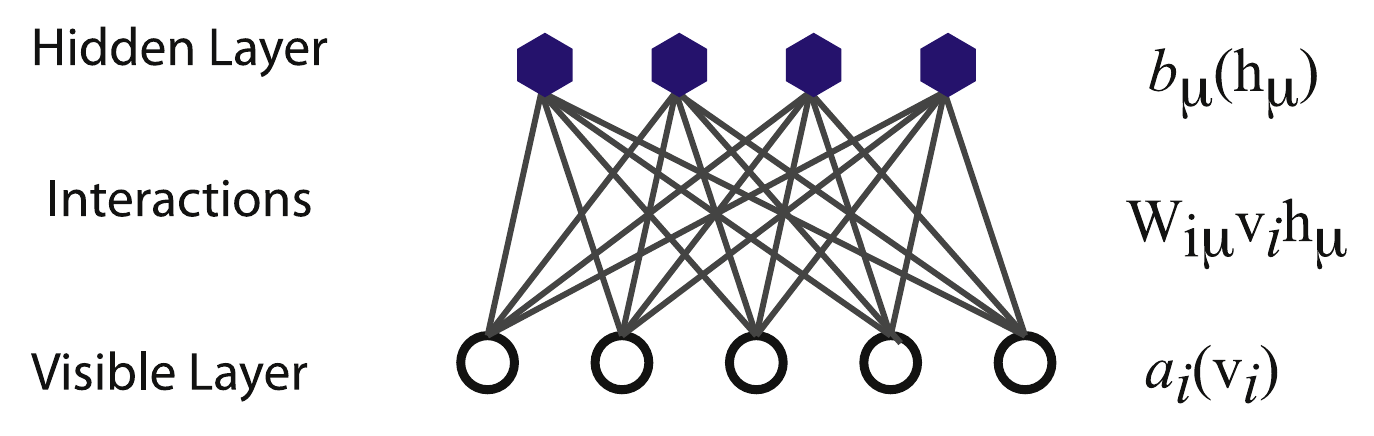
\includegraphics[width=0.44\textwidth]{RBM_structure.png}
	\caption{Bipartite structure of a Restricted Boltzmann Machine. Visible units (bottom) are connected to hidden units (top) with no intra-layer connections.}
	\label{fig:rbm_model}
\end{figure}

The probability of a hidden unit being active is computed using the logistic sigmoid for both visibile and hidden units:
\begin{equation}
	p(h_\mu=1|\mathbf{v}) = \sigma\left(b_\mu+\sum_{i}v_iw_{i\mu}\right)
	\label{eq:p_of_h}
\end{equation}
\begin{equation}
	p(v_i=1|\mathbf{h}) = \sigma\left(a_i+\sum_{\mu}h_\mu w_{i\mu}\right)
	\label{eq:p_of_v}
\end{equation}
The training consists in the minimization of the energy's $\boldsymbol{\theta}$ parameters; and is typically performed via Contrastive Divergence algorithm, which approximates the gradient of the log-likelihood by alternating Gibbs sampling between the visible and hidden layers \cite{bortoletto,practical,intro_ML}.

%%%%%%%%%%%%%%%%%%%%%%%%%%%%%%%%%%%%%%%%%%%%%%%%%%%%%%%%%%%%%%%%%%%%%%
% 3. Methodology
%%%%%%%%%%%%%%%%%%%%%%%%%%%%%%%%%%%%%%%%%%%%%%%%%%%%%%%%%%%%%%%%%%%%%%
\section{Methods}
\label{sec:methodology}

\subsection{Experimental Setup and Preprocessing}
The MNIST dataset is used, consisting of 60,000 training images and 10,000 test images of handwritten digits. Each image is flattened into a 784-dimensional vector and binarized by thresholding at 0.5. Two encoding schemes are implemented:
\begin{itemize}
	\item \textbf{Bernoulli encoding:} Pixel values in $\{0,1\}$.
	\item \textbf{Spin encoding:} Pixel values in $\{-1,+1\}$.
\end{itemize}
The RBM is implemented in a Python class (\texttt{RBM}) with configurable hyperparameters.

\subsection{Hyperparameter Tuning}
Key hyperparameters were systematically varied to assess their effect on model performance \cite{bortoletto,intro_ML,practical}. These include:
\begin{itemize}
	\item \textit{Number of hidden units (e.g., 3 to 13):} Determines the model’s capacity. Too few may lead to underfitting, while too many could cause overfitting.
	\item \textit{Contrastive Divergence (CD) steps ($k=1,2,3$):} Affects the accuracy of gradient estimation; lower $k$ may introduce bias, whereas higher $k$ could improve approximation but slows training.
	\item \textit{Learning rate and regularization coefficients:} Control the speed and stability of convergence; improper values may result in divergence or overly slow learning.
	\item \textit{Optimizer type (SGD versus RMSprop):} Influences how weights are updated and can impact convergence speed and the ability to escape local minima.
	\item \textit{Data encoding (Bernoulli vs. Spin):} Alters the energy function and conditional probabilities, affecting how well the model captures data characteristics.
\end{itemize}
For each configuration, training is repeated over multiple runs (each executed 10 times) to ensure statistically robust results.

\begin{figure}[!tb]
	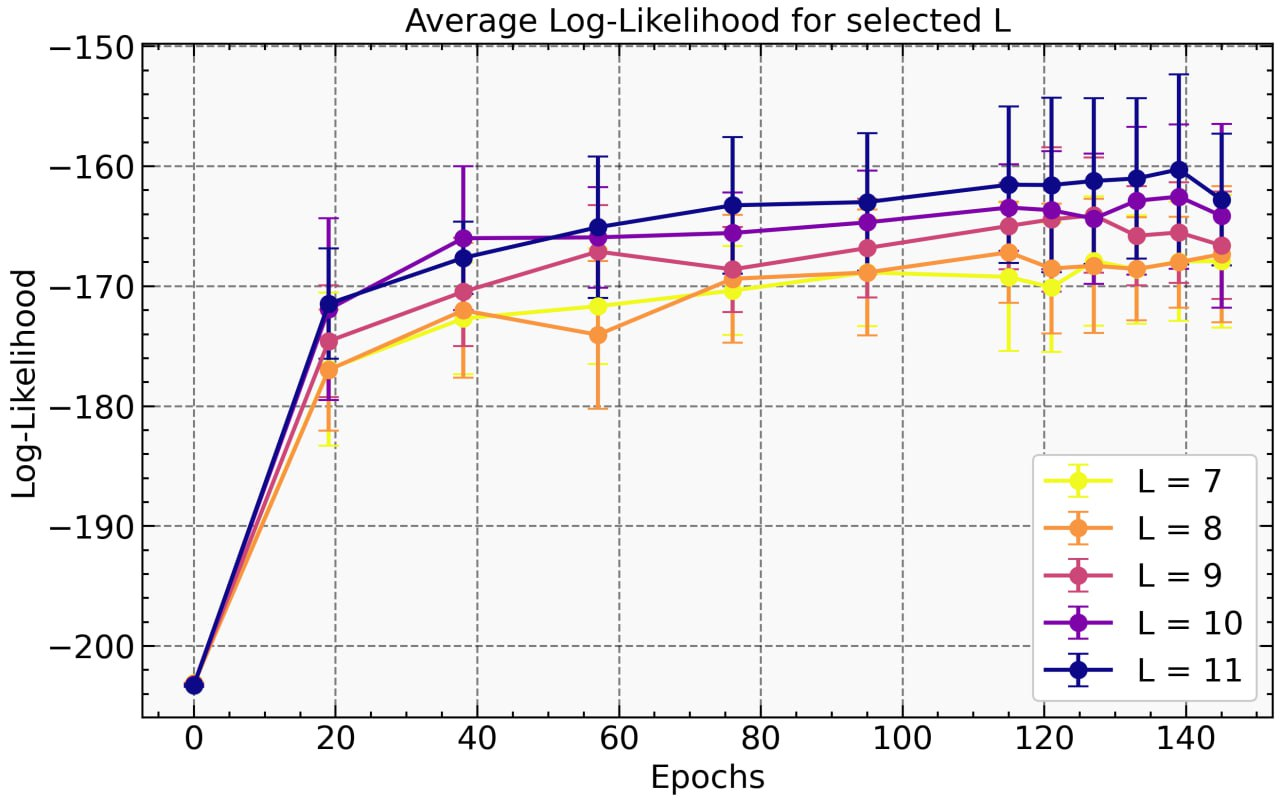
\includegraphics[width=0.44\textwidth]{L_of_epochs.jpg}
	\caption{Evolution of the log-likelihood over training epochs. Results are averaged over multiple runs.}
	\label{fig:L_of_epochs}
\end{figure}

\begin{figure}[!tb]
	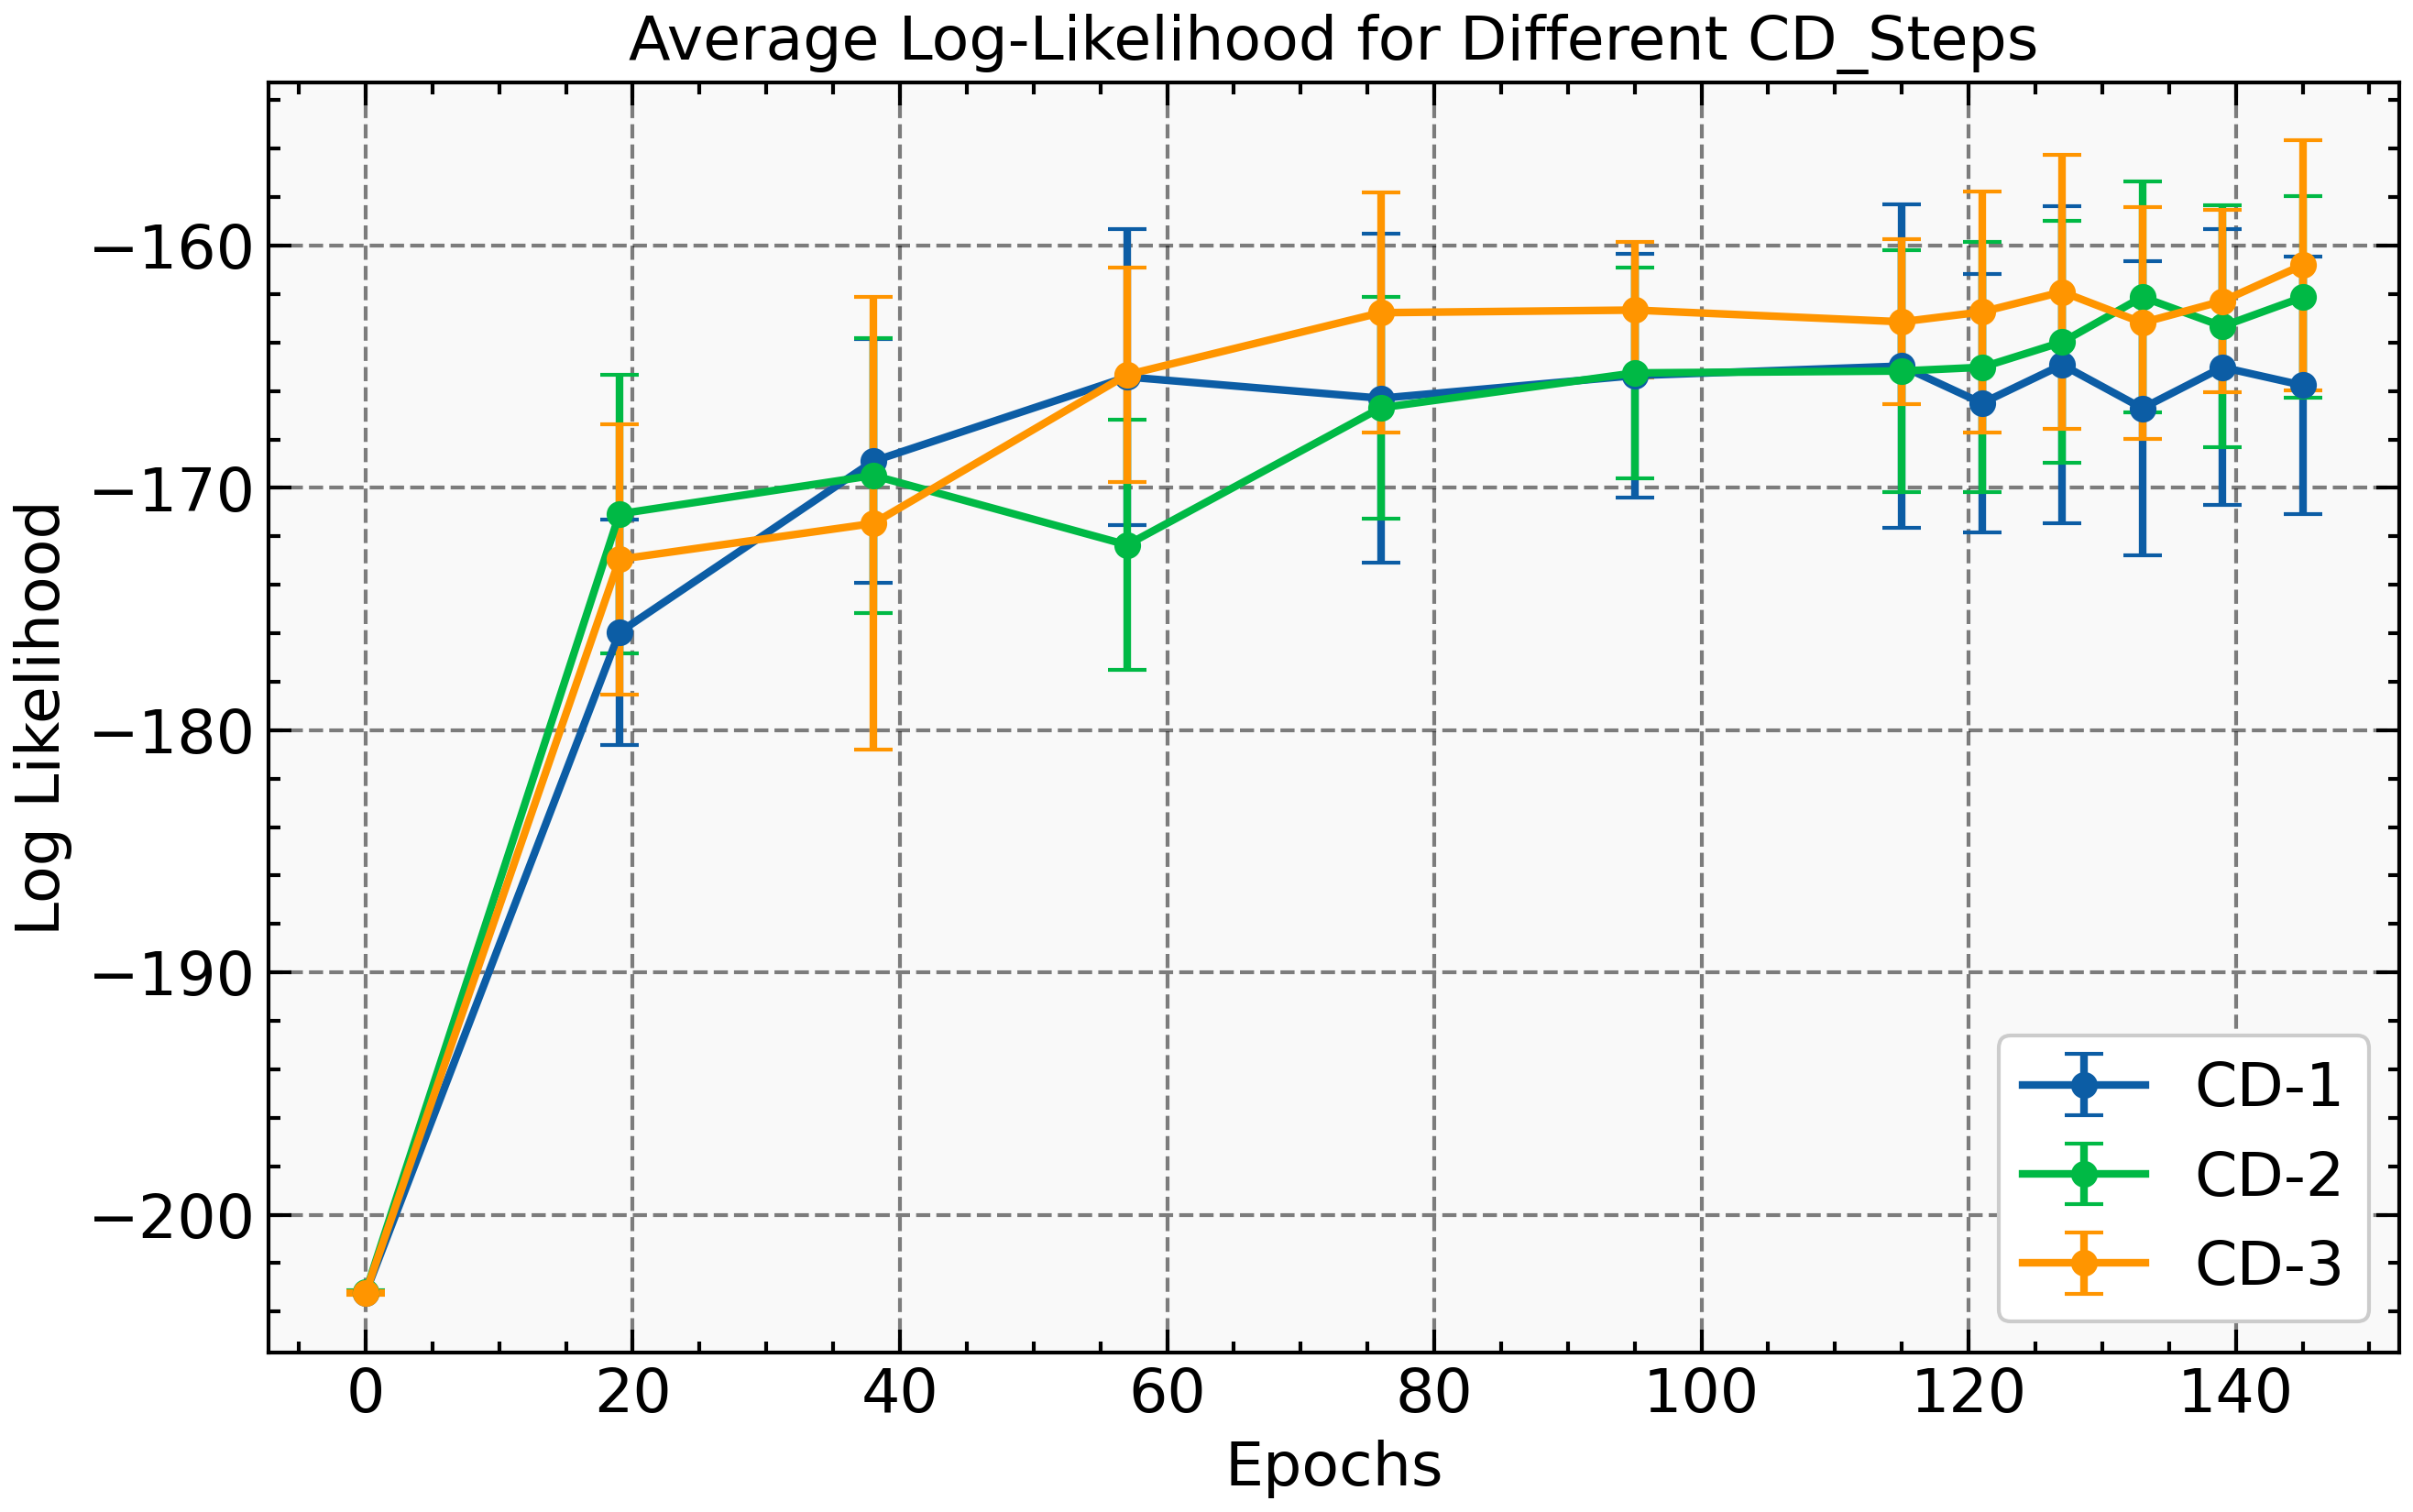
\includegraphics[width=0.44\textwidth]{L_of_CD.png}
	\caption{Log-likelihood evolution for different numbers of Contrastive Divergence steps.}
	\label{fig:L_of_CD}
\end{figure}


\subsection{Log-Likelihood Estimation}
The performance of the RBM is evaluated using the log-likelihood metric:
\begin{equation}
	\mathcal{L} = \frac{1}{M}\sum_{m=1}^{M} \log \left(\sum_{\mathbf{h}} e^{-E(\mathbf{v}^{(m)},\mathbf{h})}\right) - \log Z
	\label{eq:loglikelihood}
\end{equation}
where $Z$ is the partition function. For details control Section~\ref{sec:app}). 

%%%%%%%%%%%%%%%%%%%
\begin{figure}[!tb]
	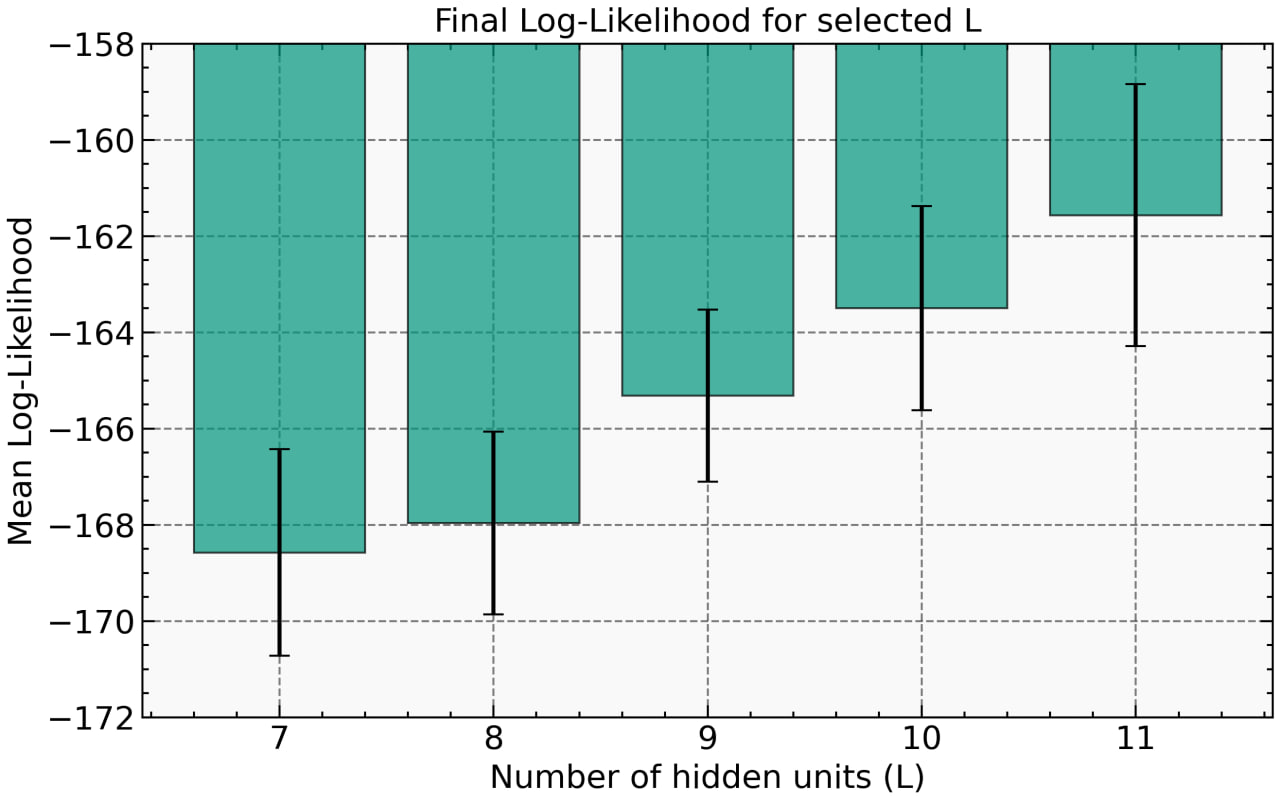
\includegraphics[width=0.44\textwidth]{L_of_L.jpg}
	\caption{Bar chart displaying the weighted mean of the log-likelihood over the last epochs for different values of L.}
	\label{fig:L_of_L}
\end{figure}
%%%%%%%%%%%%%%%%%%%

%%%%%%%%%%%%%%%%%%%
\begin{figure}[!tb]
	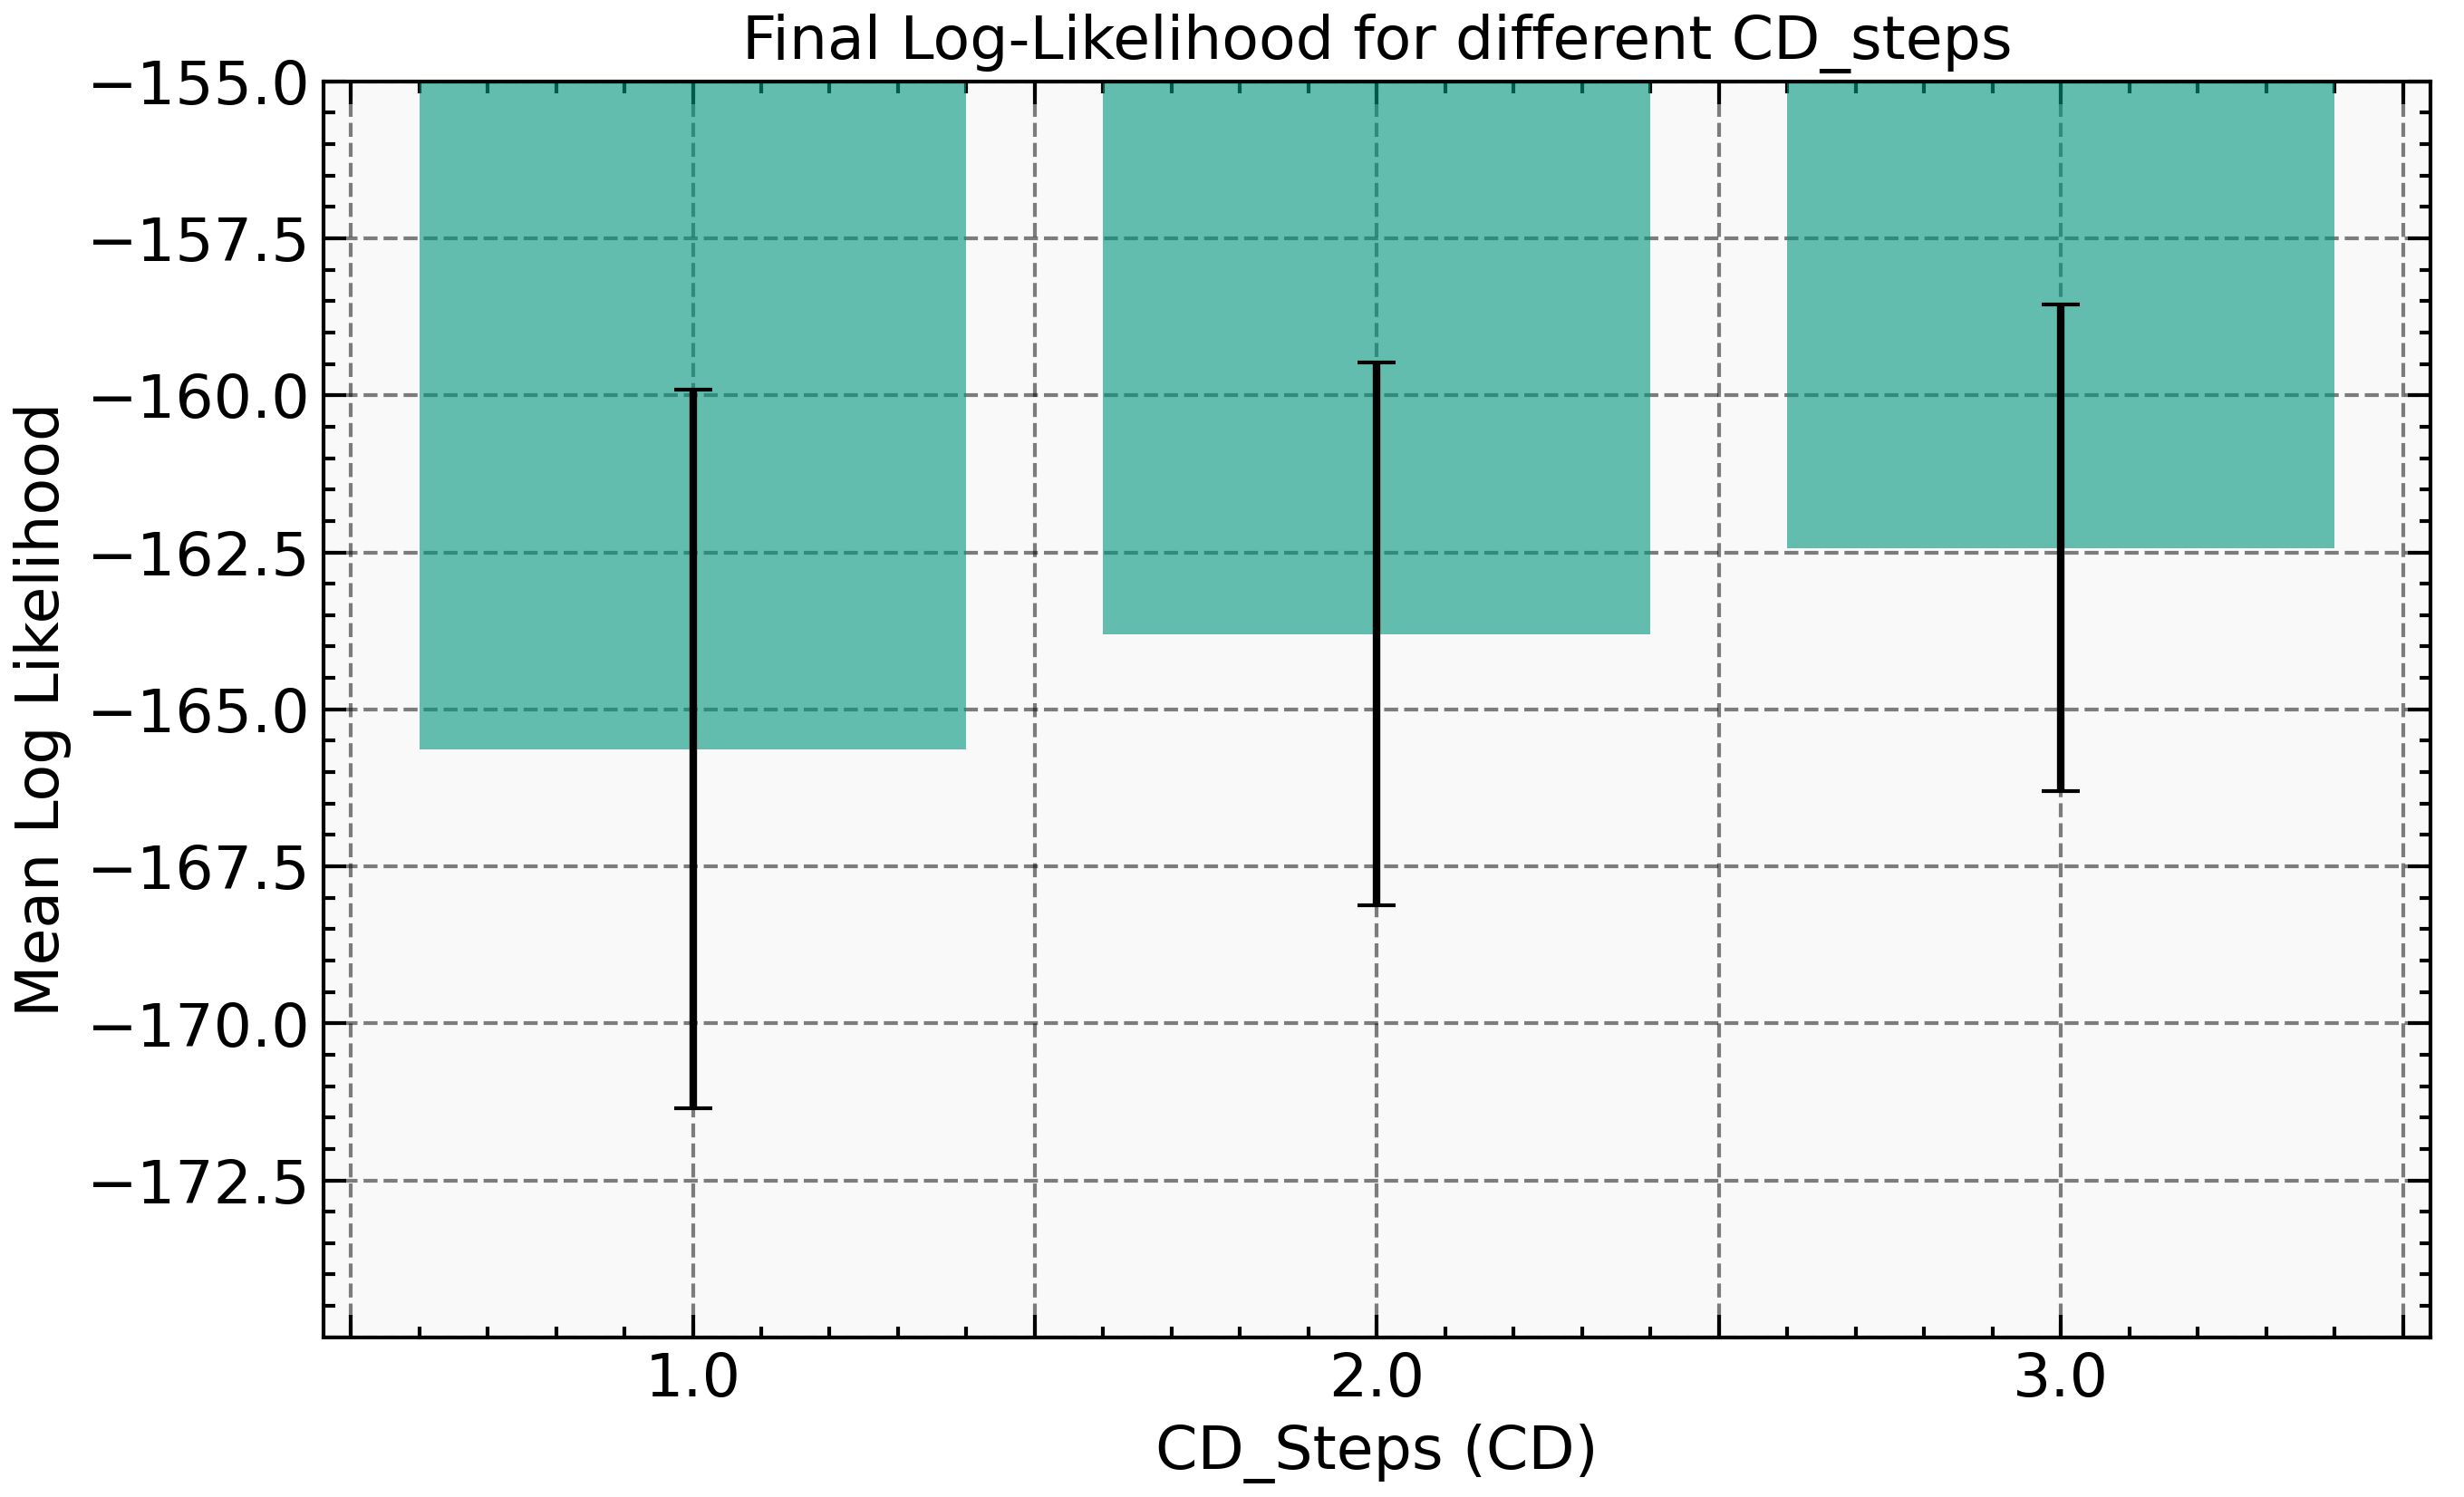
\includegraphics[width=0.465\textwidth]{final_L_of_CD.png}
	\caption{Bar chart displaying the weighted mean and standard deviation of the log-likelihood over the last epochs for different numbers of CD steps.}
	\label{fig:final_L_of_CD}
\end{figure}
%%%%%%%%%%%%%%%%%%%

This metric serves both to monitor the training progress and to ensure the consistency of the model's performance across different hyperparameter settings \cite{bortoletto,intro_ML}.

%%%%%%%%%%%%%%%%%%%%%%%%%%%%%%%%%%%%%%%%%%%%%%%%%%%%%%%%%%%%%%%%%%%%%%
% 4. Results
%%%%%%%%%%%%%%%%%%%%%%%%%%%%%%%%%%%%%%%%%%%%%%%%%%%%%%%%%%%%%%%%%%%%%%
\section{Results}
\label{sec:results}
Experimental results are presented through several graphs. IN our analysis we observed the following trends:

%%%%%%%%%%%%%%%%%%%
\begin{figure}[!tb]
	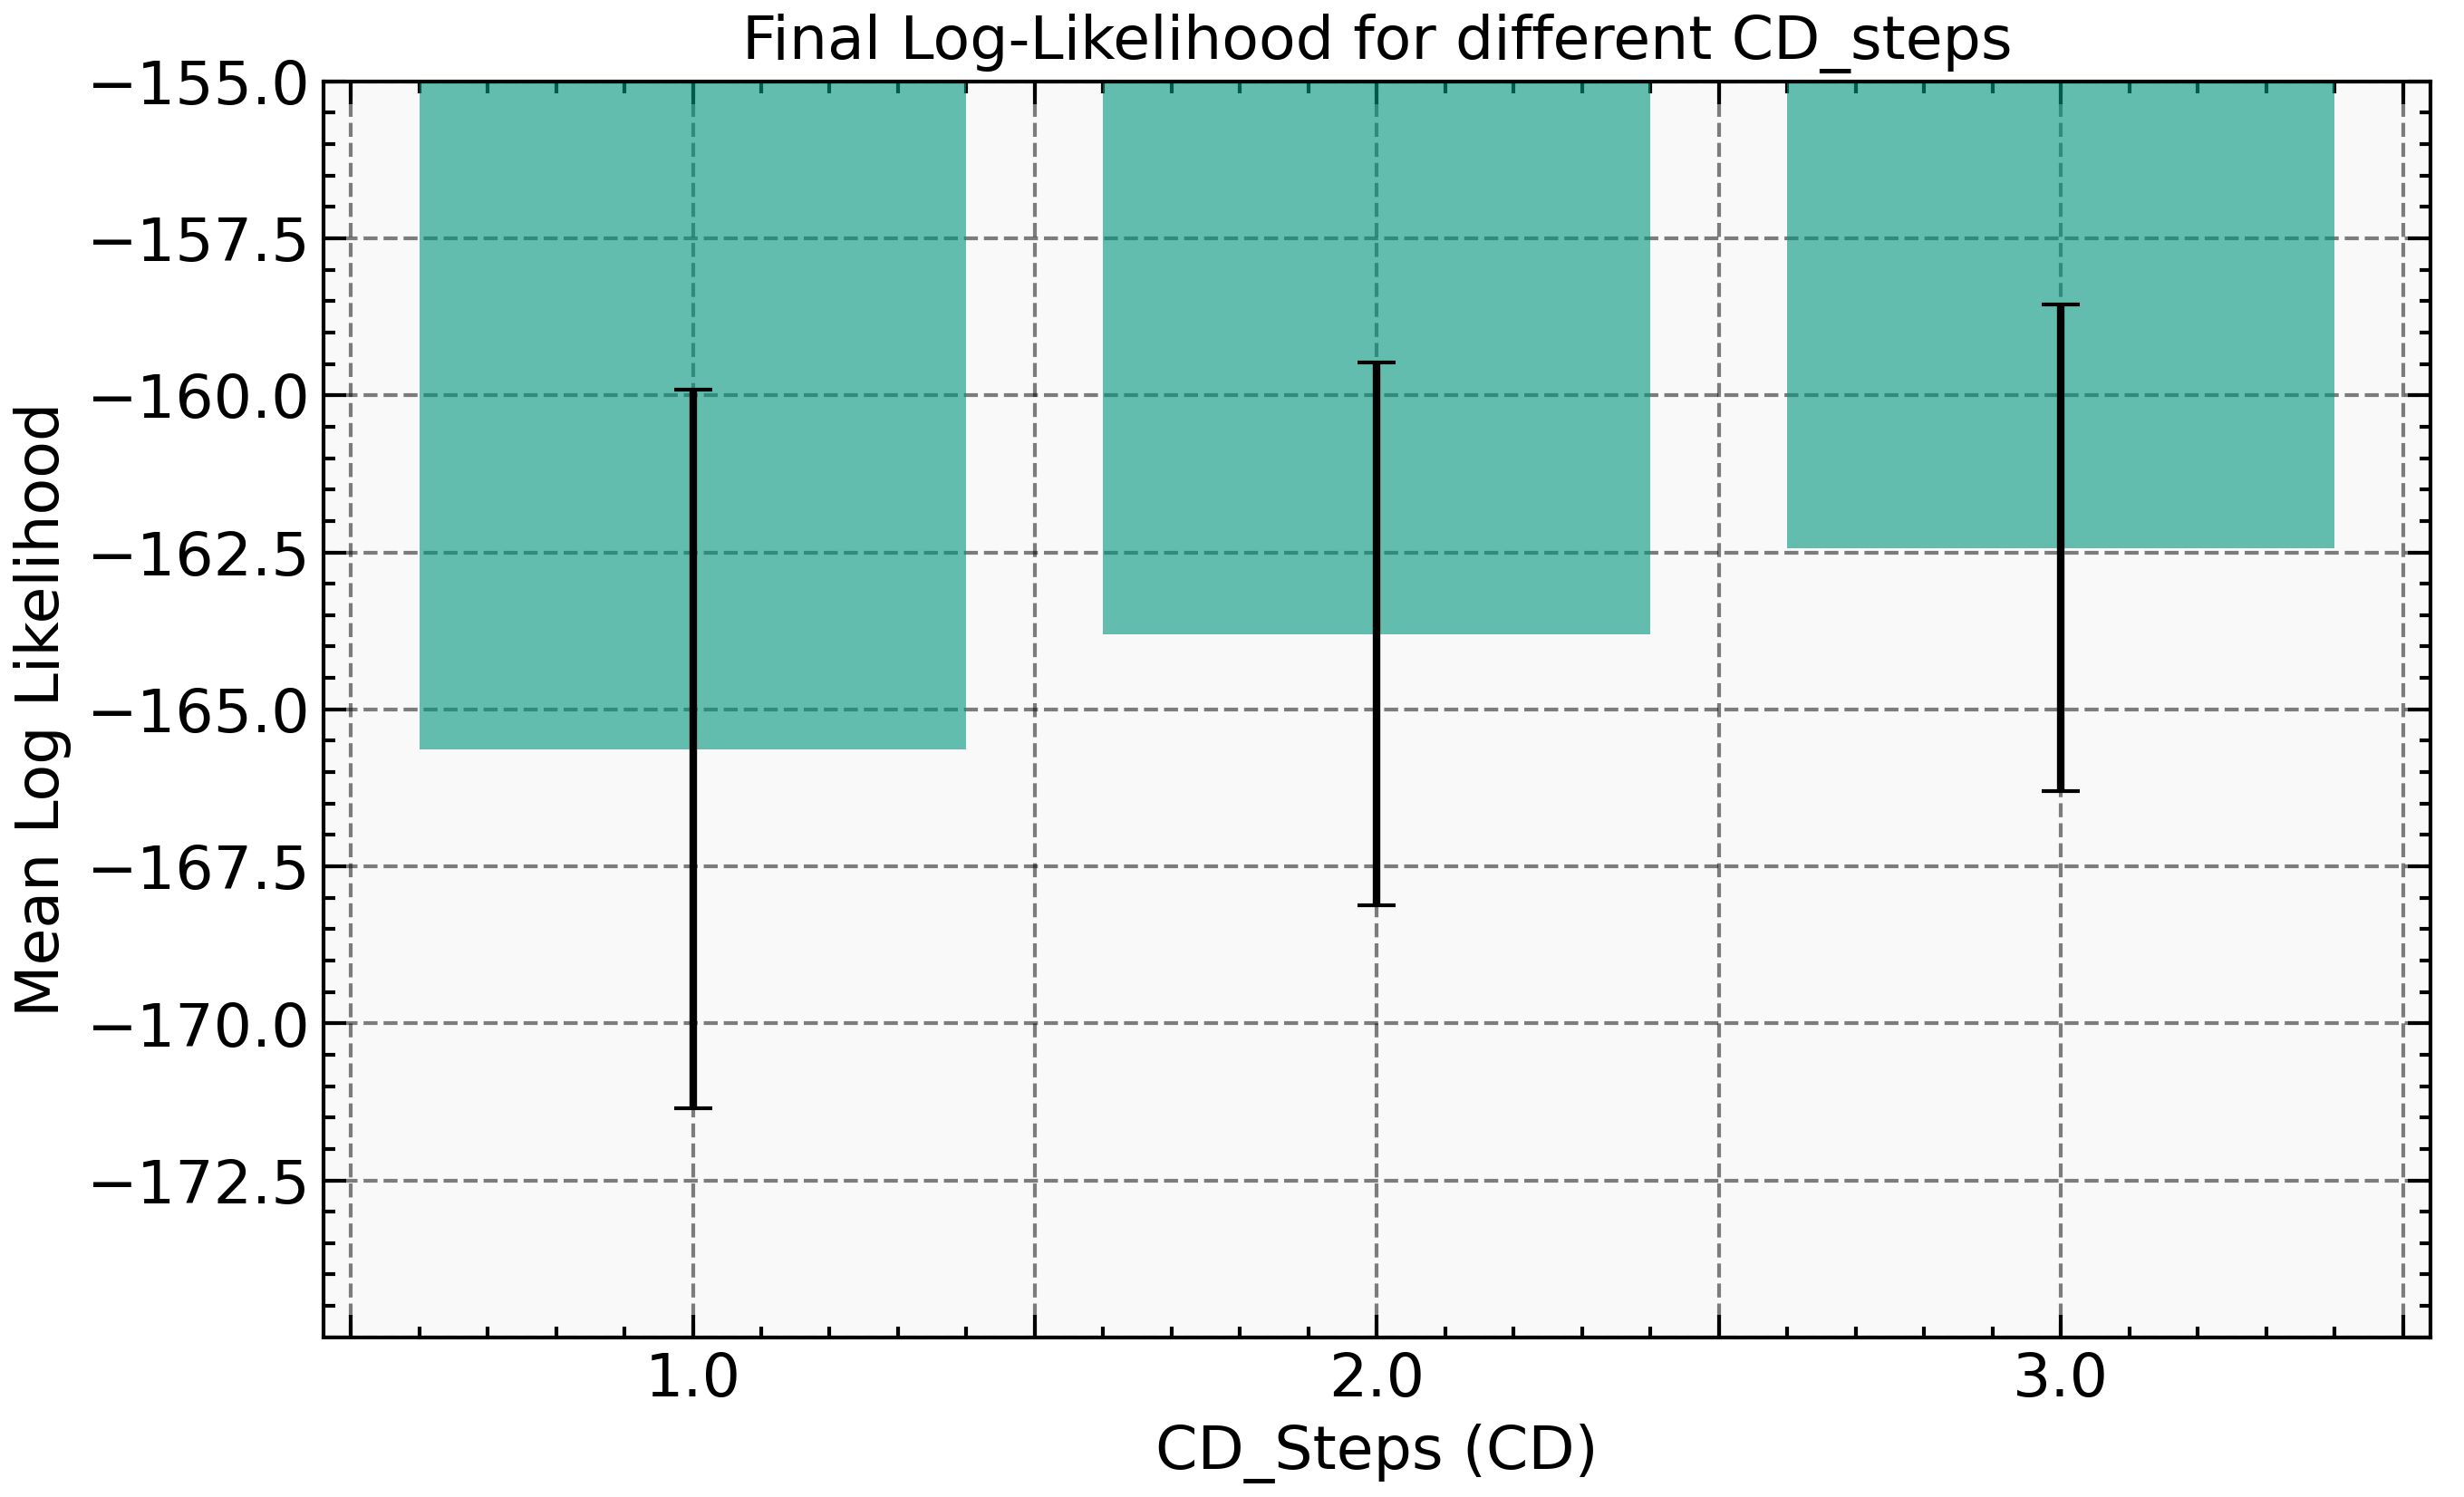
\includegraphics[width=0.465\textwidth]{final_L_of_CD.png}
	\caption{Bar chart displaying the weighted mean and standard deviation of the log-likelihood over the last epochs for different numbers of CD steps.}
	\label{fig:final_L_of_CD}
\end{figure}
%%%%%%%%%%%%%%%%%%%

%%%%%%%%%%%%%%%%%%%
\begin{figure}[!tb]
	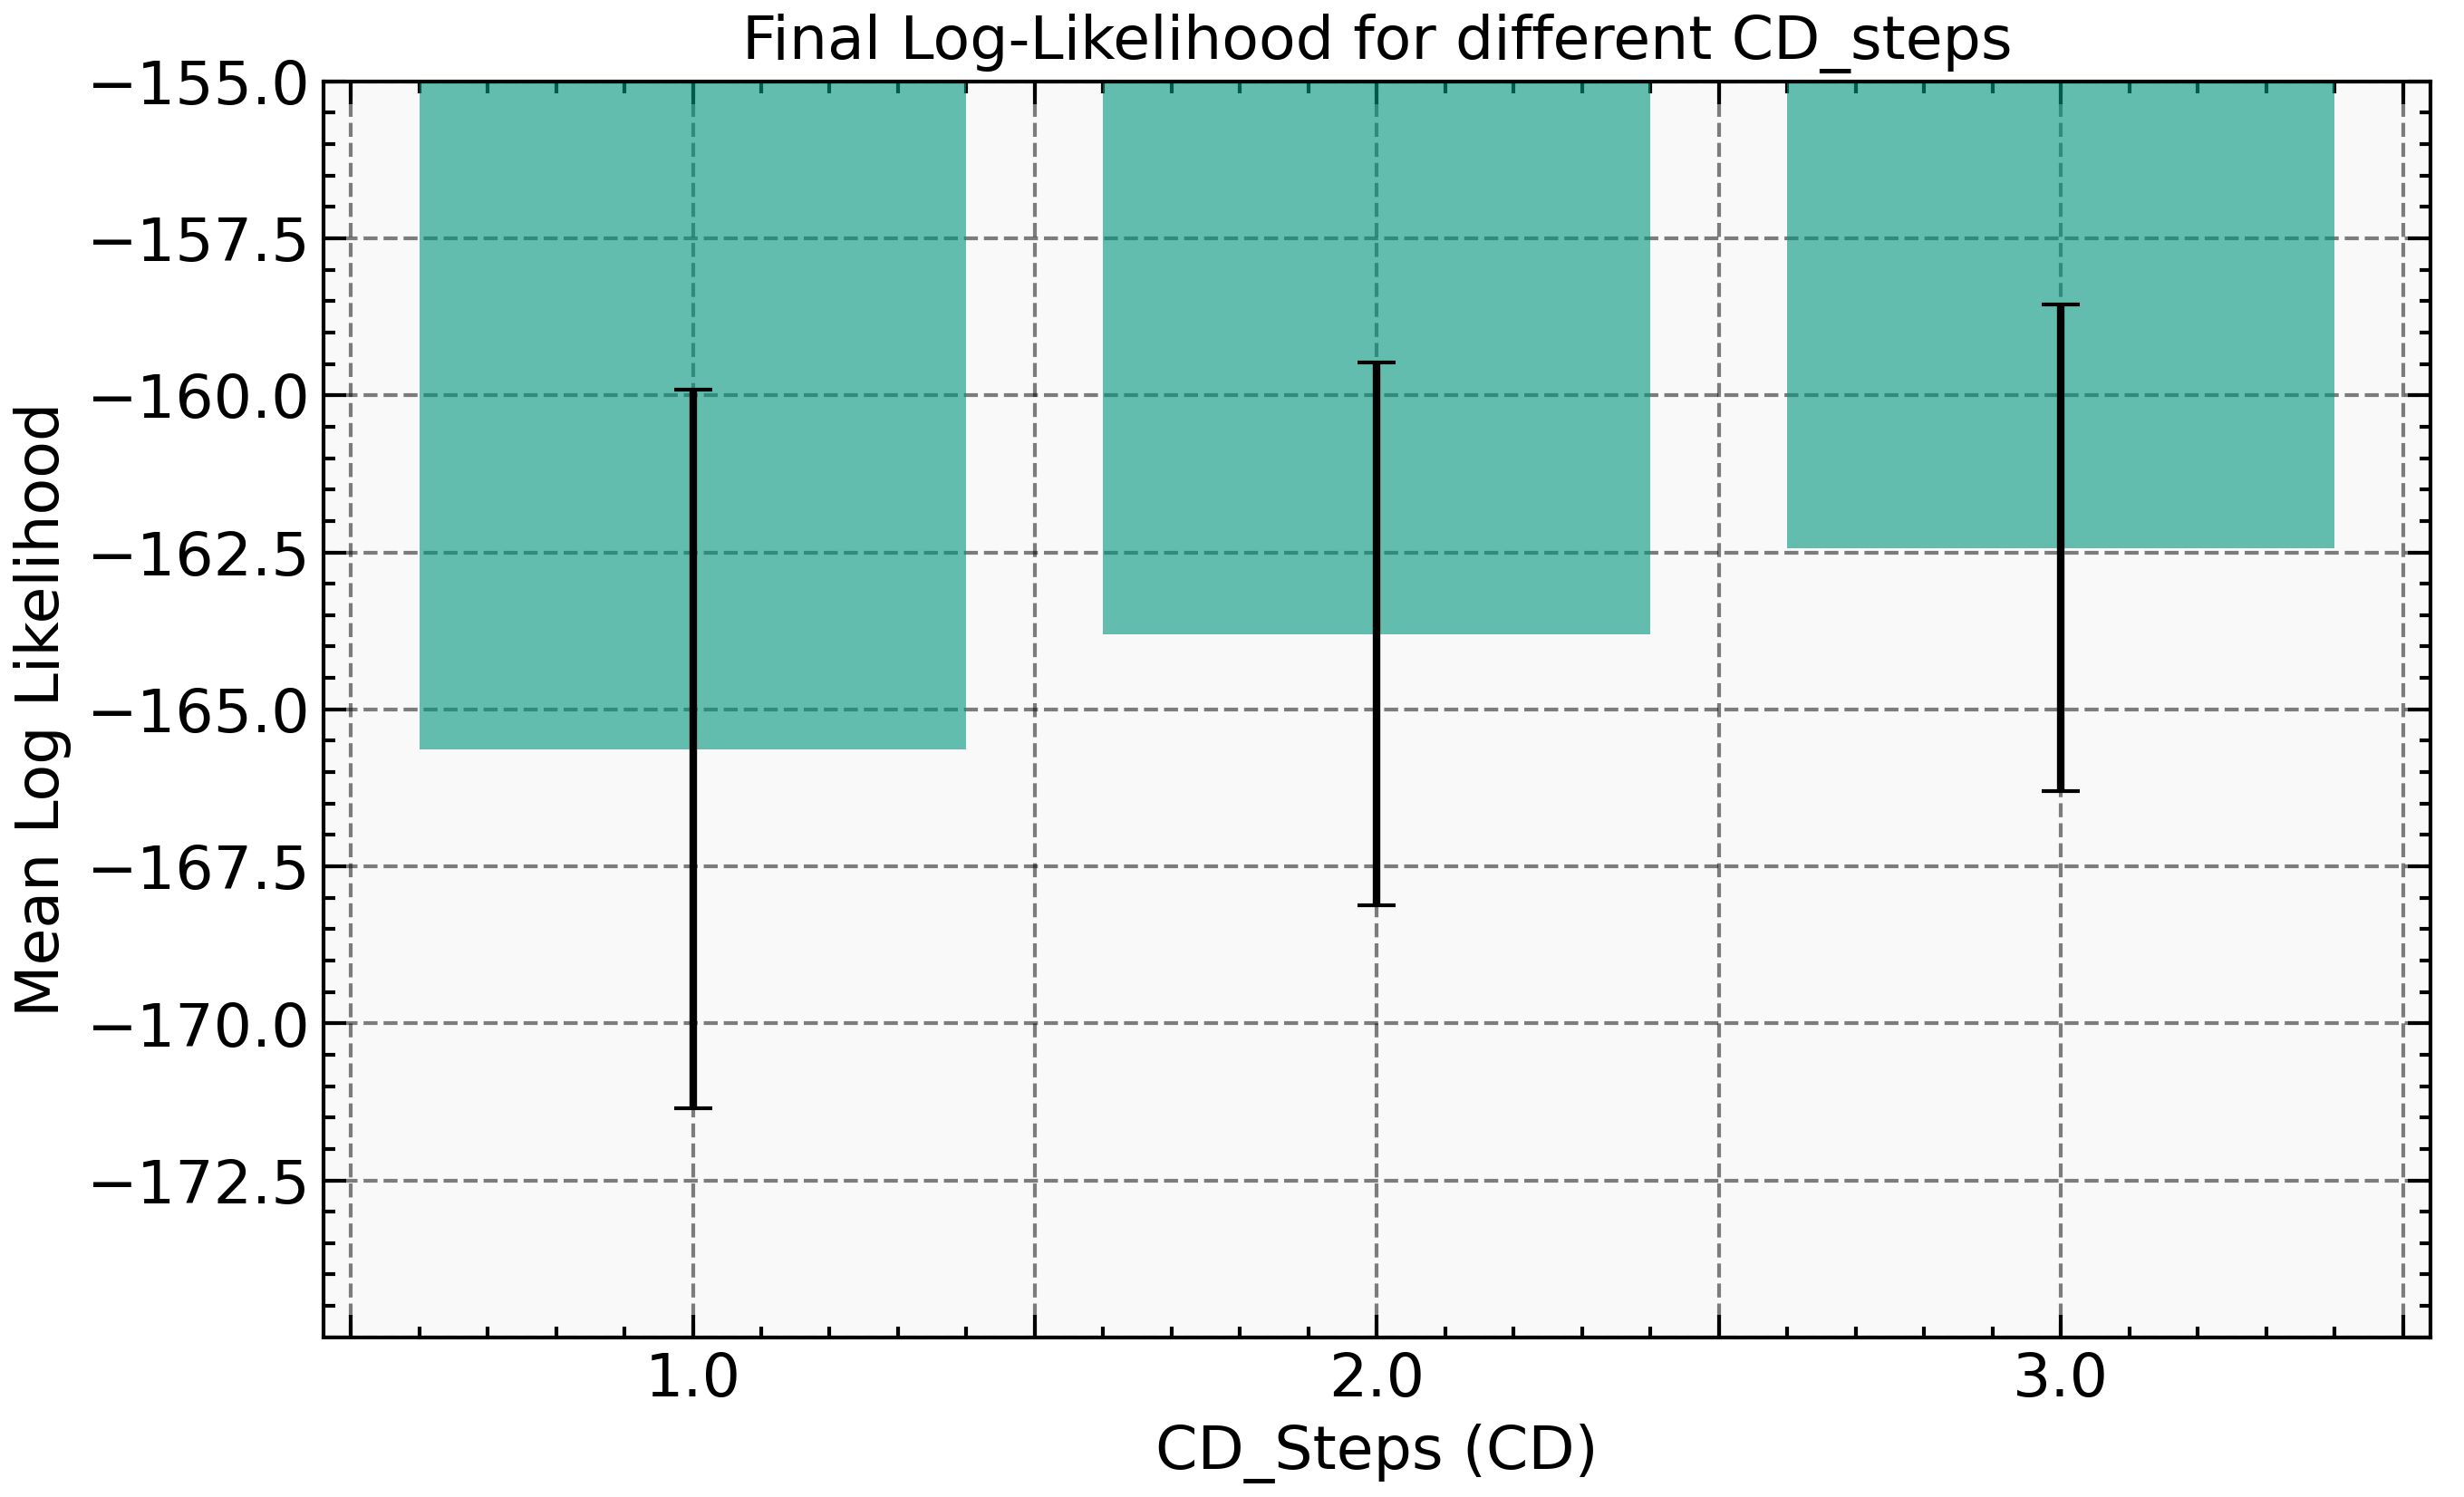
\includegraphics[width=0.465\textwidth]{final_L_of_CD.png}
	\caption{Bar chart displaying the weighted mean and standard deviation of the log-likelihood over the last epochs for different numbers of CD steps.}
	\label{fig:final_L_of_CD}
\end{figure}
%%%%%%%%%%%%%%%%%%%

\begin{itemize}
\item \textbf{Steady improvement of log-likelihood:} As depicted in Figure~\ref{fig:L_of_epochs}, the log-likelihood steadily increases during training and saturates after a sufficient number of epochs around epoch=100, confirming that the RBM is effectively learning to model the data \cite{bortoletto,practical}.
\item \textbf{Effects of CD steps:} Figure~\ref{fig:L_of_CD} indicates that increasing the number of CD steps from 1 to 3 yields only marginal gains. Moreover, the measures shows, via the analysis of the t-test after the 100 epochs, great compatibility; This suggests that CD-1 provides a good balance between computational efficiency and gradient approximation quality; however, too few steps may introduce bias and risk divergence \cite{bortoletto,practical}. For this last reason in the following tuning we kept CD-3.

%%%%%%%%%%%%%%%%%%%%%%%%%%%%%%%%%%%%%%%%%%%%%%%%%%%%%%%%%%%%%%%%%%% 
\begin{table}[!h]
	\begin{center}
		\begin{tabular}{lll}
			CD-1 vs CD-2\ \ &\ \  CD-2 vs CD-3\ \ &\ \ CD-3 vs CD-1 \\
			\hline
			$t = 0.256$ & $\ \ t = 0.236$ & $\ \ t = 0.464$
		\end{tabular}
	\end{center}
	\caption{$t$-values for each pair of chosen CD steps.}
	\label{tab:1}
\end{table}
%%%%%%%%%%%%%%%%%%%%%%%%%%%%%%%%%%%%%%%%%%%%%%%%%%%%%%%%%%%%%%%%%%%

\item
\textbf{Impact of hidden unit count:} As shown in Figure~\ref{fig:L_of_L}, increasing the number of hidden units improves performance up to a point, after which the benefits plateau. This reflects the model's ability to capture data complexity without incurring overfitting when the capacity is appropriately chosen \cite{bortoletto,practical}.
\item
\textbf{Influence of activation and encoding schemes:} Our experiments also reveal that one-hot hidden activations (POTS) and spin encoding can lead to instability or degraded performance, highlighting the importance of selecting appropriate unit types and data representations for stable learning \cite{bortoletto,practical}.
\end{itemize}

%%%%%%%%%%%%%%%%%%%
\begin{figure}[!tb]
	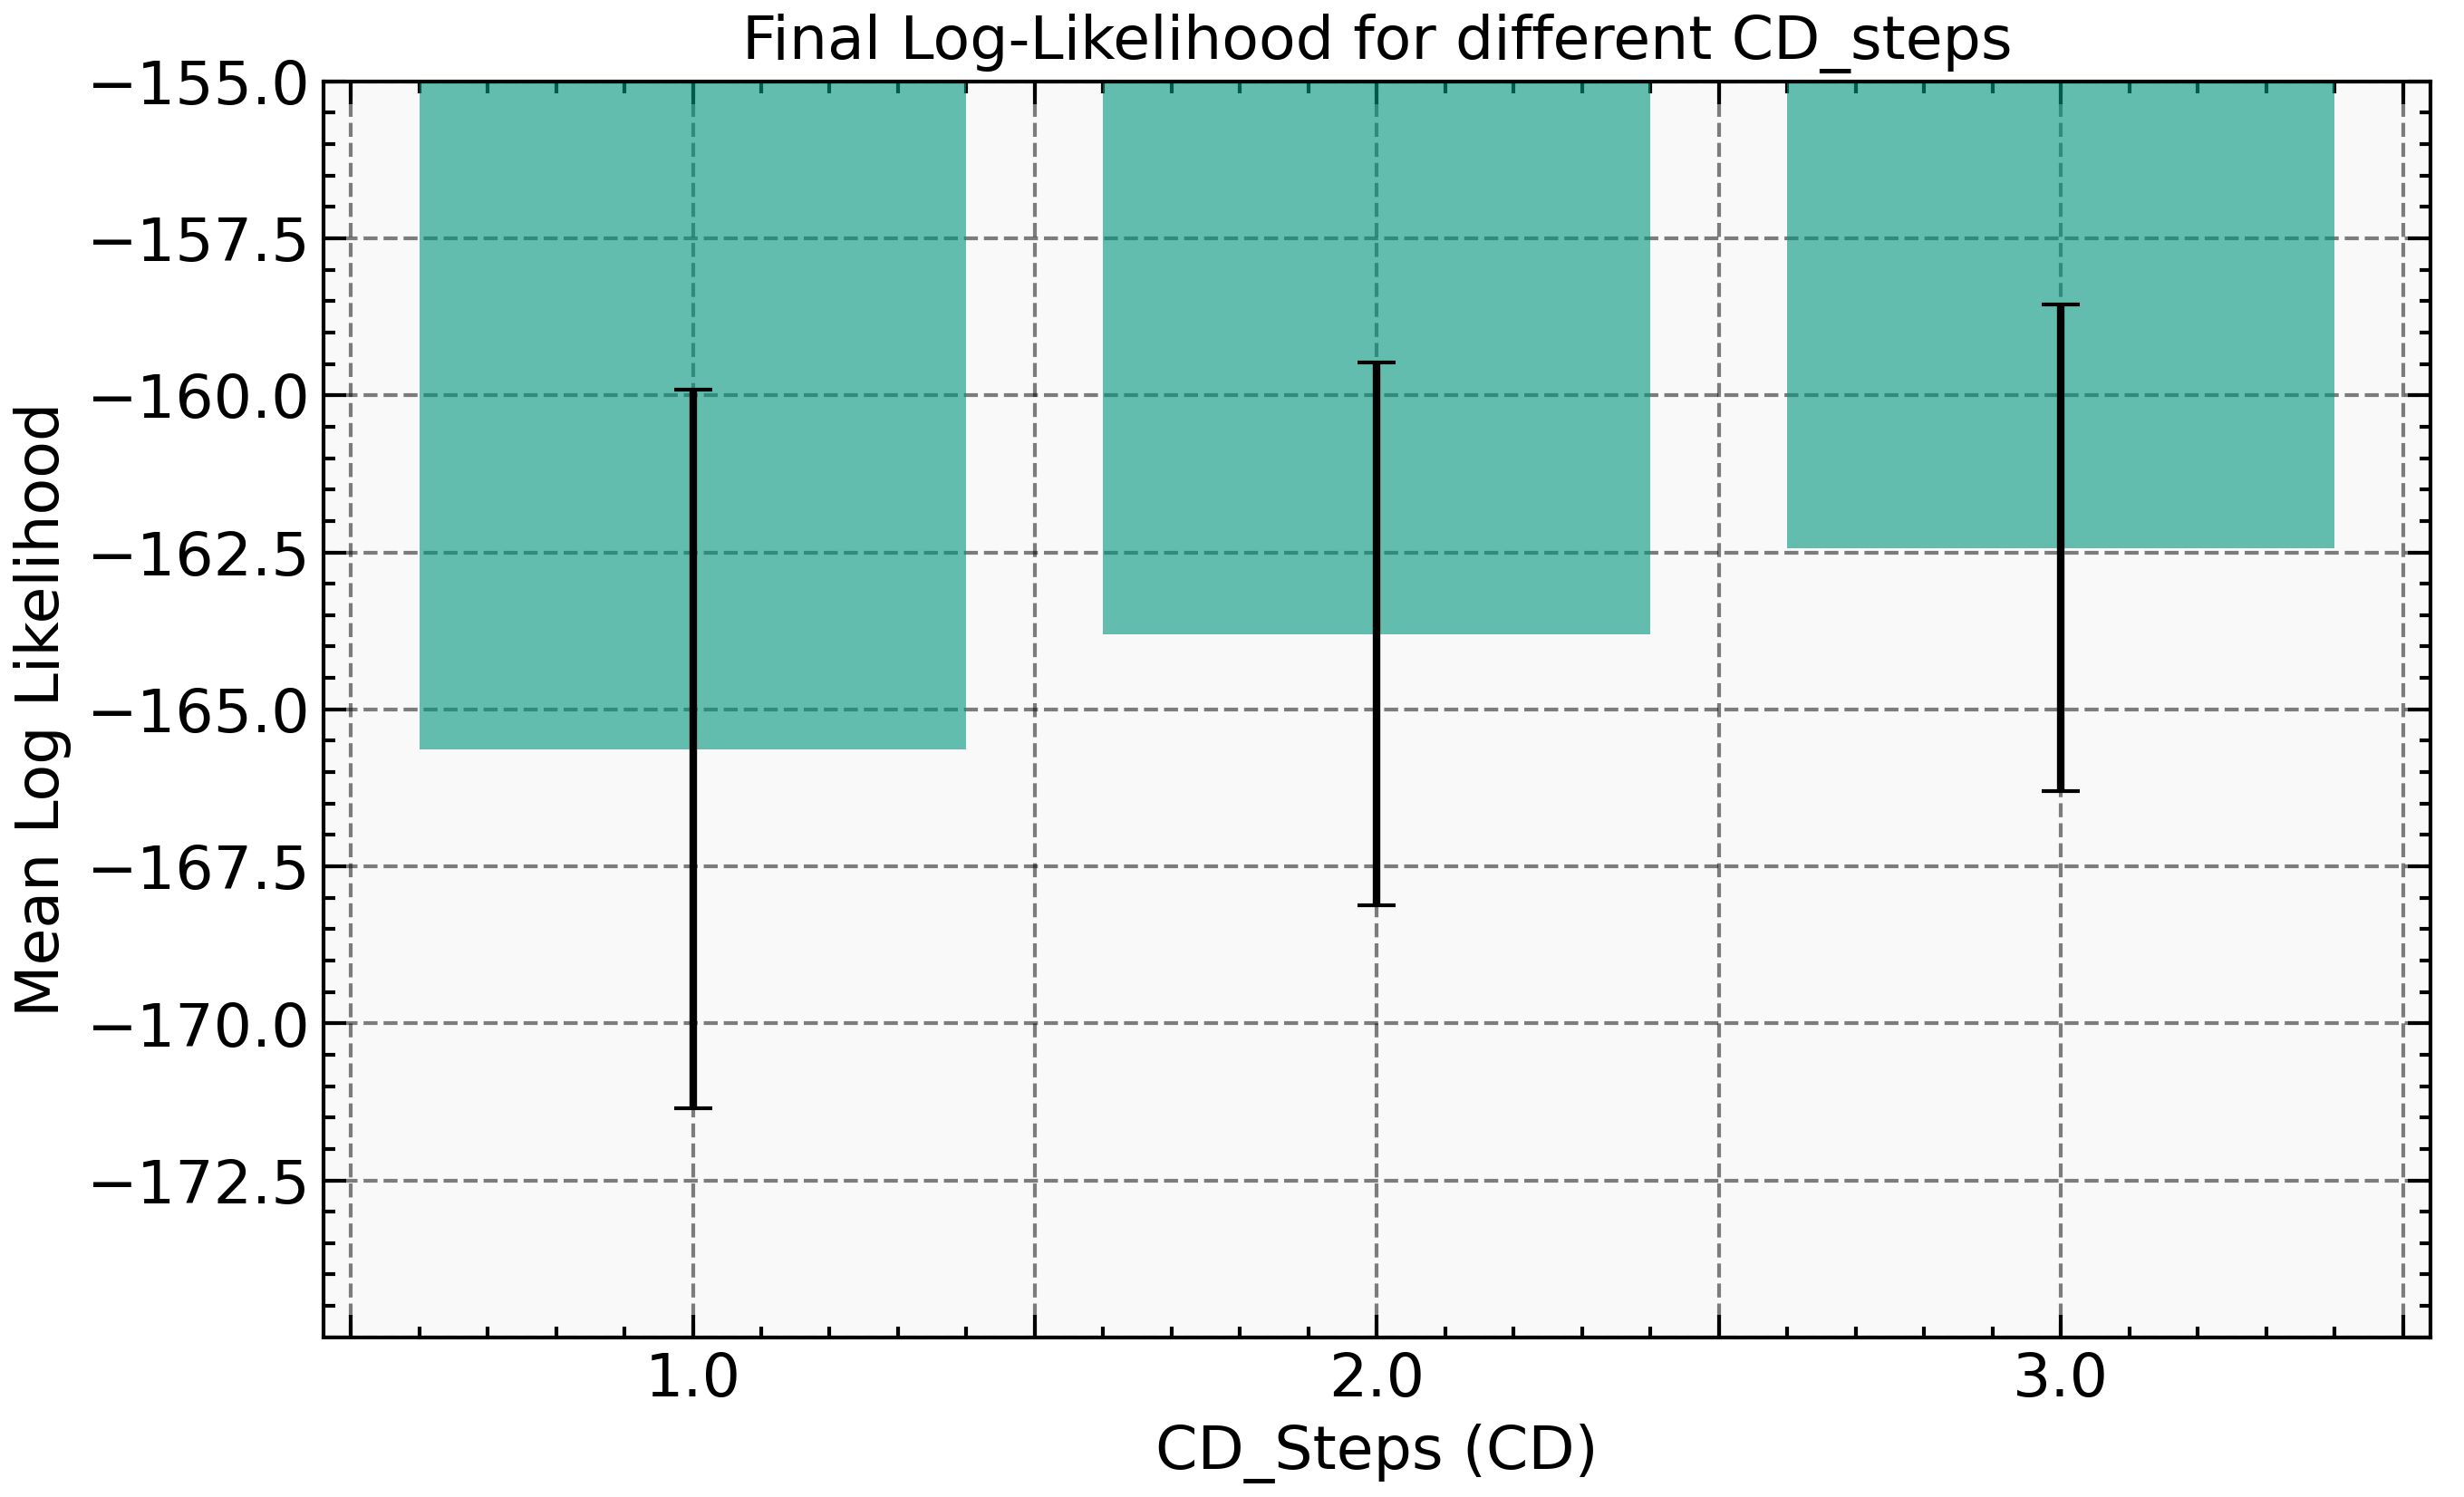
\includegraphics[width=0.465\textwidth]{final_L_of_CD.png}
	\caption{Bar chart displaying the weighted mean and standard deviation of the log-likelihood over the last epochs for different numbers of CD steps.}
	\label{fig:final_L_of_CD}
\end{figure}
%%%%%%%%%%%%%%%%%%%

%%%%%%%%%%%%%%%%%%%
\begin{figure}[!tb]
	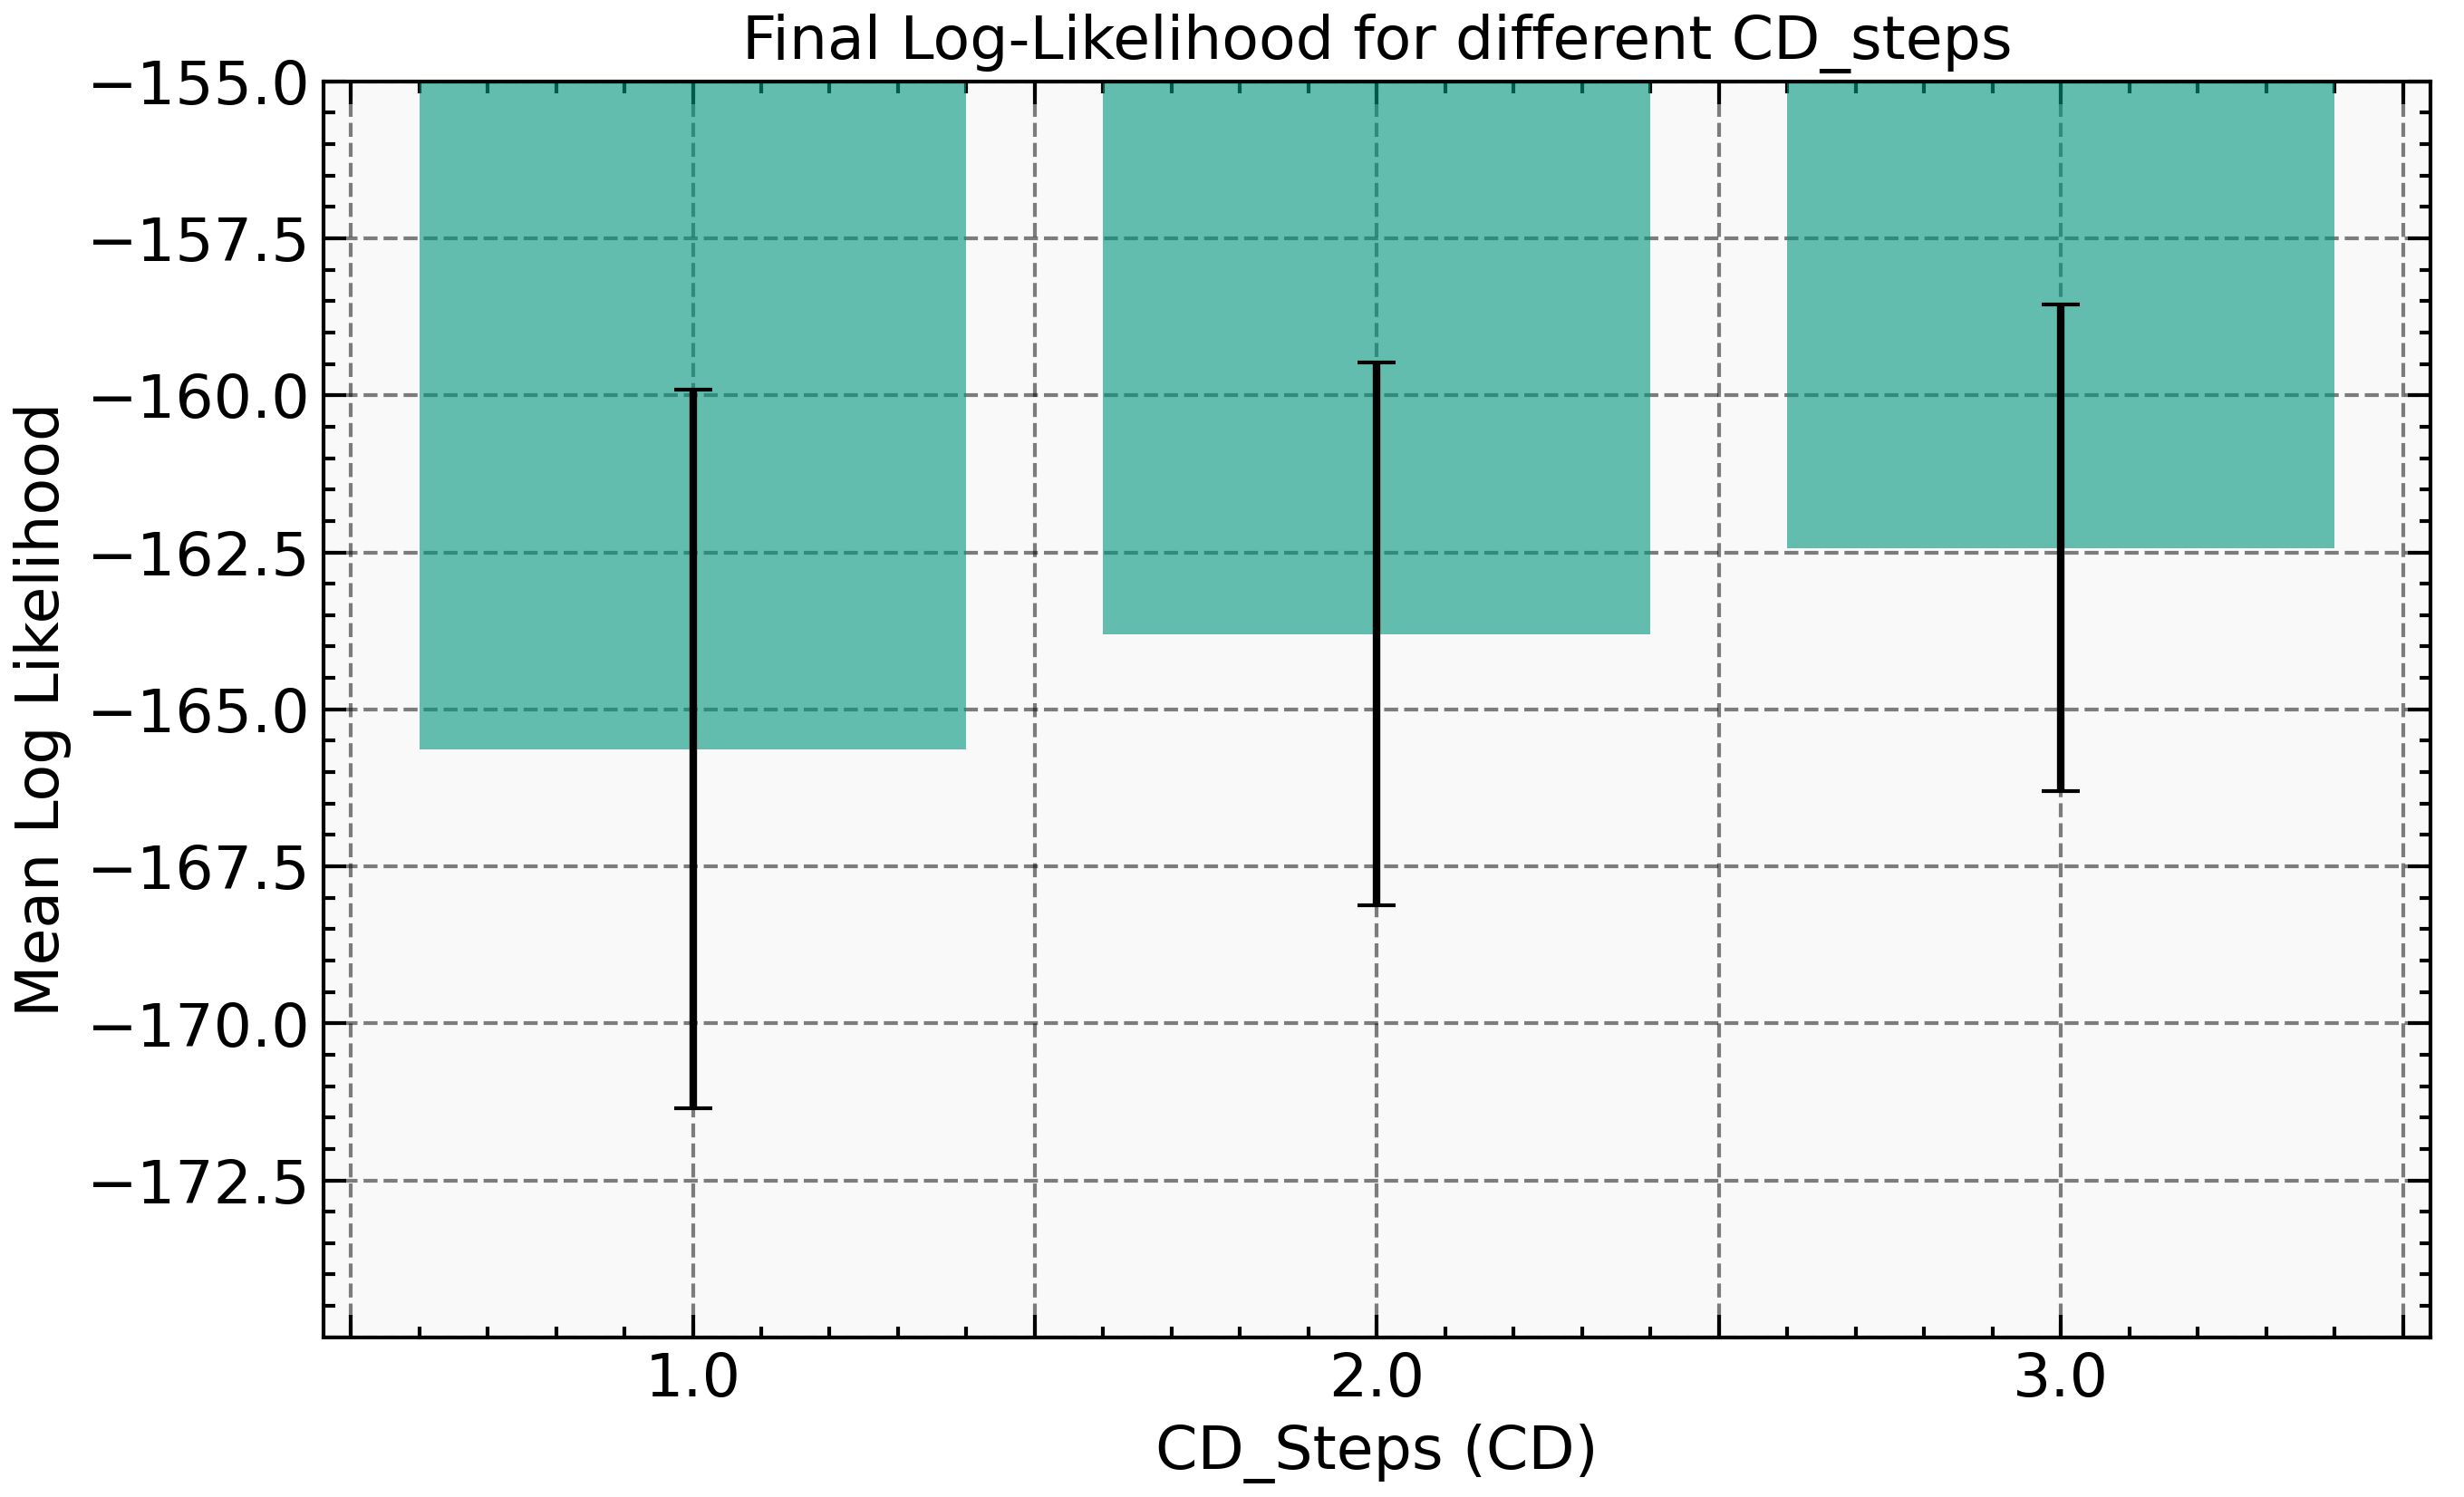
\includegraphics[width=0.465\textwidth]{final_L_of_CD.png}
	\caption{Bar chart displaying the weighted mean and standard deviation of the log-likelihood over the last epochs for different numbers of CD steps.}
	\label{fig:final_L_of_CD}
\end{figure}
%%%%%%%%%%%%%%%%%%%

%%%%%%%%%%%%%%%%%%%%%%%%%%%%%%%%%%%%%%%%%%%%%%%%%%%%%%%%%%%%%%%%%%%%%%
% 5. Discussion and Conclusion
%%%%%%%%%%%%%%%%%%%%%%%%%%%%%%%%%%%%%%%%%%%%%%%%%%%%%%%%%%%%%%%%%%%%%%
\section{Discussion and Conclusion}
\label{sec:discussion}
Our experiments confirm that RBMs are capable of learning useful representations of handwritten digits in an unsupervised fashion. The analysis shows that:
\begin{itemize}
	\item Proper initialization and regularization are critical for stable training.
	\item While increasing hidden units improves performance, the benefit saturates beyond a certain network capacity.
	\item The choice of optimizer and data encoding significantly affects convergence dynamics.
\end{itemize}
These findings provide a baseline for further research, which might include adaptive scheduling of CD steps, deeper architectures (e.g., stacked RBMs), or alternative estimation techniques (such as AIS). Overall, the work not only demonstrates the practical viability of RBMs but also highlights their limitations and areas for future improvement.

%%%%%%%%%%%%%%%%%%%%%%%%%%%%%%%%%%%%%%%%%%%%%%%%%%%%%%%%%%%%%%%%%%%%%%
% 6. Appendix
%%%%%%%%%%%%%%%%%%%%%%%%%%%%%%%%%%%%%%%%%%%%%%%%%%%%%%%%%%%%%%%%%%%%%%
\section{Appendix}
\label{sec:app}
\subsection*{Gradient Update Equations and Regularization}
\begin{equation}
	\boldsymbol{\theta}_{t+1}=\boldsymbol{\theta}_t-\gamma\cdot\eta_t\cdot\text{sign}(\boldsymbol{\theta})
	\label{eq:regu}
\end{equation}
\begin{equation}
	\boldsymbol{\theta}_{t+1}=\boldsymbol{\theta}_t\pm\eta_t\cdot{}\nabla_{\boldsymbol{\theta}}E(\boldsymbol{\theta})
	\label{eq:sgd}
\end{equation}
\begin{equation}
	\begin{cases}
		\boldsymbol{g}_t=\nabla_{\boldsymbol{\theta}}E(\boldsymbol{\theta}) \\
		\boldsymbol{s}_t=\beta\boldsymbol{s}_{t-1}+(1-\beta)\boldsymbol{g}_t^2 \\
		\boldsymbol{\theta}_{t+1}=\boldsymbol{\theta}_t\pm\eta_t\frac{\boldsymbol{g}_t}{\sqrt{\boldsymbol{s}_t+\epsilon}}
	\end{cases}
	\label{eq:rmsprop}
\end{equation}

\subsection*{Log-Likelihood and Partition Function Approximations}

The log-likelihood $\mathcal{L}$ of the data is defined as
\begin{equation}
	\mathcal{L} = \frac{1}{M}\sum_{m=1}^{M} \ell_{\theta}(v^{(m)})
	\label{eq:Loglikelihood}
\end{equation}
with
\begin{equation}
	\ell_{\theta}(v^{(m)}) = \log \sum_{h} e^{-E(v^{(m)},h)} - \log Z
	\label{eq:loglikelihood}
\end{equation}
Here, $M$ is the number of data points and $Z$ denotes the partition function. The energy function $E(v,h)$ is expressed through
\begin{equation}
	e^{-E(v,h)} = G(h)\prod_{i} e^{H_i(h)v_i}
\end{equation}
where
\begin{equation}
	G(h) = \prod_{\mu} e^{b_{\mu}h_{\mu}} \quad \text{and} \quad H_i(h) = a_i + \sum_{\mu} w_{i\mu}h_\mu
\end{equation}
In Equation~\ref{eq:loglikelihood}, the summation over $h$ runs over all possible states of the hidden layer.

Since directly computing the partition function $Z$ is computationally intractable, we apply approximations and normalization techniques. A more in-depth mathematical analysis about this procedure can be found in \cite{baiesi}.

For the Bernoulli encoding, the partition function is manipulated as:
\begin{equation}
	Z = q^D\sum_{h} G(h) \prod_{i=1}^D \frac{1+e^{H_i(h)}}{q}
	\label{eq:Z_function_bernulli}
\end{equation}
where $q$ is a scaling factor introduced to avoid numerical overflow. For spin encoding, where the units assume values in $\{-1,1\}$, the partition function is approximated by
\begin{equation}
	Z = \sum_{h} G(h) \prod_{i=1}^D 2\cdot{}\cosh\left(H_i(h)\right)
	\label{eq:Z_function_spin}
\end{equation}

In eq.~\ref{eq:Z_function_spin}, to ensure numerical stability, we relaborated the product introducing a logaritm to avoid overflow.
The product becomes via \textit{logarithmic identity}:
   \begin{equation}
   \log\left(\prod_{i=1}^N 2\cdot{}\cosh(x_i)\right) = \underbrace{N\cdot{}\log(2)}_{\text{from } 2^N} +\sum_{i=1}^N \log\left(\cosh(x_i)\right)
   \end{equation}
   we compute this sum instead of multiplying large values directly.

Where the log(cosh) is manipulated using the identity
   \begin{equation}
   \log(\cosh(x)) = |x| - \log(2) + \log\left(1 + e^{-2|x|}\right)
   \end{equation}
   which avoids overflow and underflow. In Python we used \textsc{numpy.log1p} for precision.
 The sum over \( \log(2\cosh(x_i)) \) becomes:
\begin{equation}
\begin{split}
\sum_{i=1}^N \log(2\cosh(x_i)) = \sum_{i=1}^N \left[\log(2) + \log(\cosh(x_i))\right] \\
= \underbrace{N\log(2)}_{\text{explicit } \log(2)} + \sum_{i=1}^N \left[|x_i| - \log(2) + \log\left(1 + e^{-2|x_i|}\right)\right]
\end{split}
\end{equation}
The \( N\log(2) \) term cancels out, leaving:
\begin{equation}
\sum_{i=1}^N \left(|x_i| + \log\left(1 + e^{-2|x_i|}\right)\right)
\end{equation}
That we used in our algorithm to ensure numerical stability.
% Bibliography
\bibliography{biblio}
\bibliographystyle{apsrev4-1}

\end{document}